\documentclass[11pt]{article}
\usepackage{anysize} 
\marginsize{2cm}{2cm}{2cm}{2cm} 

\usepackage{multirow}
\usepackage{tabularx}
\usepackage{longtable}
\usepackage[utf8]{inputenc}
\usepackage[spanish]{babel}
\usepackage{hyperref}
\usepackage{fixltx2e}
\usepackage{mathtools}
\usepackage{amsmath}
\usepackage{graphicx}
\usepackage{adjustbox}
\usepackage{subcaption}
\usepackage{floatrow}

%%%%%%%%%%%%%%%%%%%%%%%%%%%%%%%%%%%%%%%%%%%%%%%%%
%	headers & footers							%
%%%%%%%%%%%%%%%%%%%%%%%%%%%%%%%%%%%%%%%%%%%%%%%%%
\usepackage{fancyhdr}
\pagestyle{fancy}
\fancyhf{}
\rhead{Taller de Sistemas Computacionales}
\lhead{Segundo Semestre 2014}
\rfoot{Página \thepage}

%%%%%%%%%%%%%%%%%%%%%%%%%%%%%%%%%%%%%%%%%%%%%%%%%
%	comandos									%
%%%%%%%%%%%%%%%%%%%%%%%%%%%%%%%%%%%%%%%%%%%%%%%%%

\newcommand{\labno}{3}
\newcommand{\labtitle}{Taller de Sistemas Computacionales}
\newcommand{\nameone}{Iván González López}
\newcommand{\emailone}{ivan.gonzalezlo@alumnos.usm.cl}
\newcommand{\rolone}{2973523-9}
\newcommand{\nametwo}{Guillermo Baeza Figueroa}
\newcommand{\emailtwo}{guillermo.baeza@alumnos.usm.cl}
\newcommand{\roltwo}{2973600-6}


%%%%%%%%%%%%%%%%%%%%%%%%%%%%%%%%%%%%%%%%%%%%%%%%%
%	documento									%
%%%%%%%%%%%%%%%%%%%%%%%%%%%%%%%%%%%%%%%%%%%%%%%%%


\begin{document}
\begin{titlepage}
\begin{center}

%%%%%%%%%%%%%%%%%%%%%%%%%%%%%%%%%%%%%%%%%%%%%%%%%
%	título página inicial						%
%%%%%%%%%%%%%%%%%%%%%%%%%%%%%%%%%%%%%%%%%%%%%%%%%


\includegraphics[width=70pt]{logos/utfsm.pdf} \\
{\Large \textsc{Universidad Técnica Federico Santa María} \\}
{\Large \textsc{Departamento de Informática} \\ \vspace{4pt}}
{\rule[13pt]{\textwidth}{1pt} \\ \vspace{25pt}}
{\LARGE \textsc{Tarea No. \labno} \\}
{\LARGE \textsc{\labtitle} \\ \vspace{50pt}}

%%%%%%%%%%%%%%%%%%%%%%%%%%%%%%%%%%%%%%%%%%%%%%%%%
%	autores										%
%%%%%%%%%%%%%%%%%%%%%%%%%%%%%%%%%%%%%%%%%%%%%%%%%
\begin{minipage}{0.4\textwidth}
\begin{flushleft}
{\large \nameone} \\
\emailone \\
\rolone
\end{flushleft}
\end{minipage}
\hfill
\begin{minipage}{0.4\textwidth}
\begin{flushright}
{\large \nametwo} \\
\emailtwo \\
\roltwo
\end{flushright}
\end{minipage}
\end{center}
\end{titlepage}


\section{Descripción}

\section{Análisis y Desarrollo}
\subsection{Instalación httpd}
\begin{figure}[ht]
\floatbox[{\capbeside\thisfloatsetup{capbesideposition={right,top},capbesidewidth=7cm}}]{figure}[\FBwidth]
{\caption{Repositorios de descarga de paquetes de CentOs}\label{fig:repositorios}}
{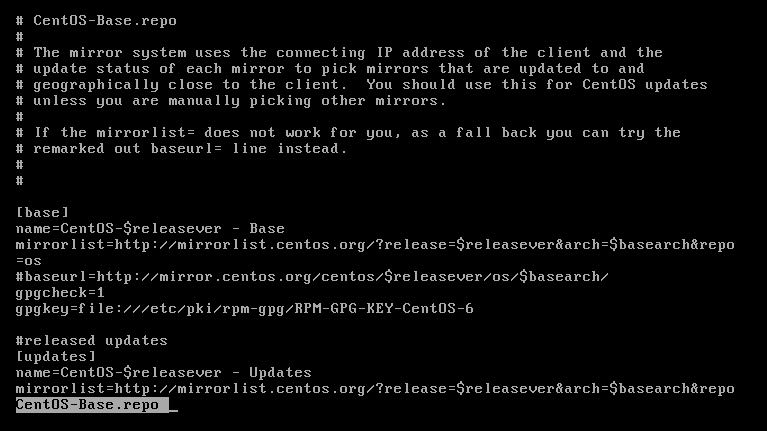
\includegraphics[width=10cm]{screenshots/httpd-install/repositorios-centos.png}}
\end{figure}

\begin{figure}[ht]
\floatbox[{\capbeside\thisfloatsetup{capbesideposition={right,top},capbesidewidth=7cm}}]{figure}[\FBwidth]
{\caption{Repositorios de descarga de paquetes de CentOs}\label{fig:repositorios}}
{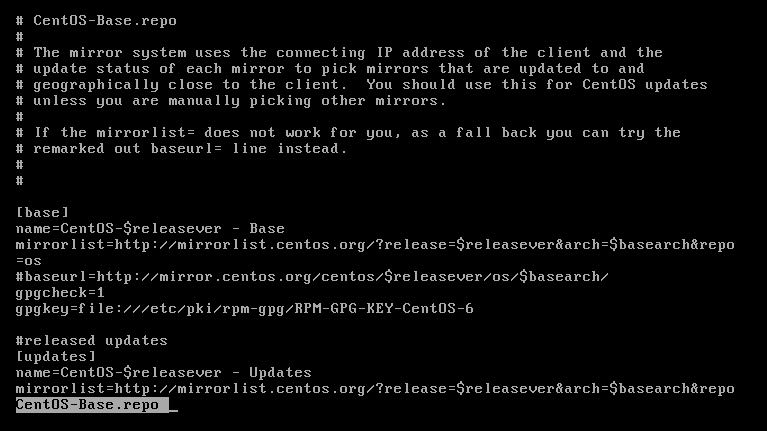
\includegraphics[width=10cm]{screenshots/httpd-install/repositorios-centos.png}}
\end{figure}

\begin{figure}[ht]
\floatbox[{\capbeside\thisfloatsetup{capbesideposition={right,top},capbesidewidth=7cm}}]{figure}[\FBwidth]
{\caption{Repositorios de descarga de paquetes de CentOs}\label{fig:repositorios}}
{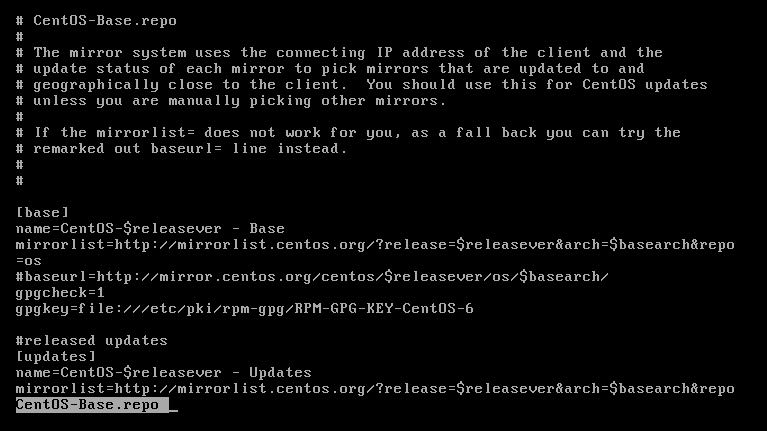
\includegraphics[width=10cm]{screenshots/httpd-install/repositorios-centos.png}}
\end{figure}

\begin{figure}[ht]
\floatbox[{\capbeside\thisfloatsetup{capbesideposition={right,top},capbesidewidth=7cm}}]{figure}[\FBwidth]
{\caption{Repositorios de descarga de paquetes de CentOs}\label{fig:repositorios}}
{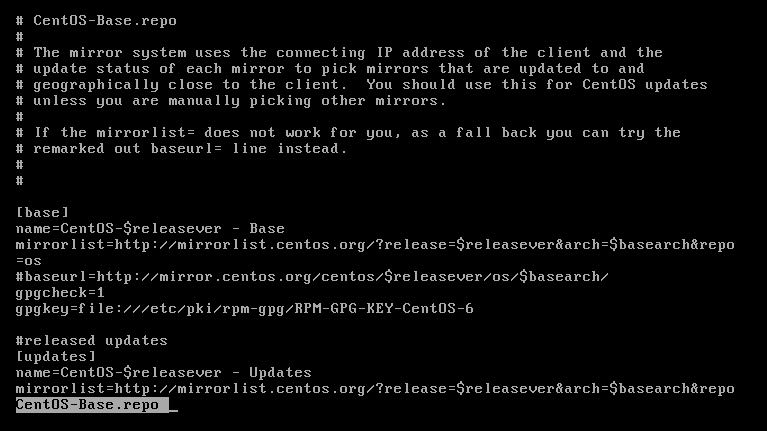
\includegraphics[width=10cm]{screenshots/httpd-install/repositorios-centos.png}}
\end{figure}

\begin{figure}[ht]
\floatbox[{\capbeside\thisfloatsetup{capbesideposition={right,top},capbesidewidth=7cm}}]{figure}[\FBwidth]
{\caption{Repositorios de descarga de paquetes de CentOs}\label{fig:repositorios}}
{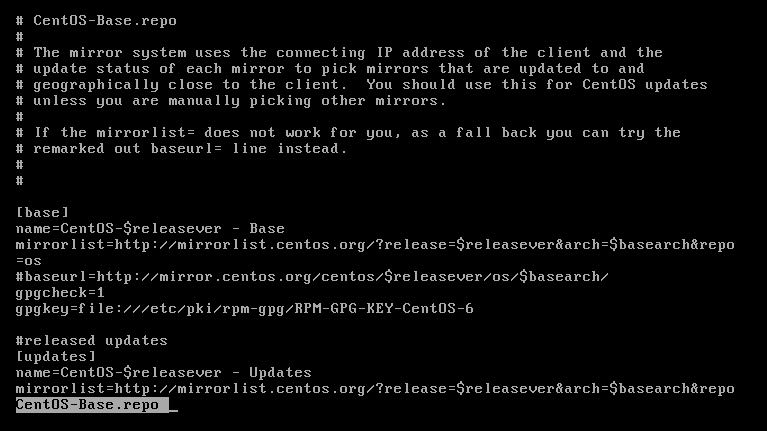
\includegraphics[width=10cm]{screenshots/httpd-install/repositorios-centos.png}}
\end{figure}

\begin{figure}[ht]
\floatbox[{\capbeside\thisfloatsetup{capbesideposition={right,top},capbesidewidth=7cm}}]{figure}[\FBwidth]
{\caption{Repositorios de descarga de paquetes de CentOs}\label{fig:repositorios}}
{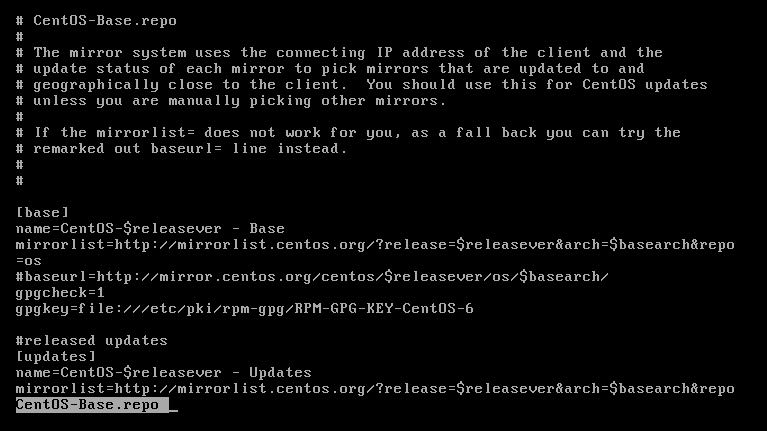
\includegraphics[width=10cm]{screenshots/httpd-install/repositorios-centos.png}}
\end{figure}

\begin{figure}[ht]
\floatbox[{\capbeside\thisfloatsetup{capbesideposition={right,top},capbesidewidth=7cm}}]{figure}[\FBwidth]
{\caption{Repositorios de descarga de paquetes de CentOs}\label{fig:repositorios}}
{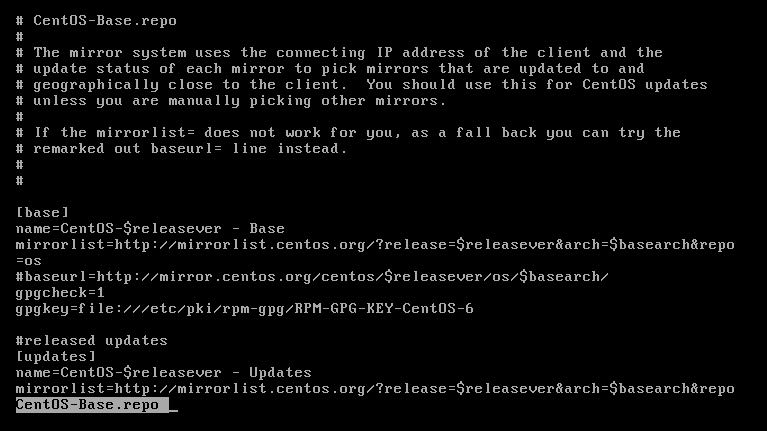
\includegraphics[width=10cm]{screenshots/httpd-install/repositorios-centos.png}}
\end{figure}


\end{document}
